% Created 2021-03-03 Wed 14:38
% Intended LaTeX compiler: pdflatex
\documentclass[english]{article}
\usepackage[T1, T2A]{fontenc}
\usepackage[lutf8]{luainputenc}
\usepackage[english, russian]{babel}
\usepackage{minted}
\usepackage{graphicx}
\usepackage{longtable}
\usepackage{hyperref}
\usepackage{xcolor}
\usepackage{natbib}
\usepackage{amssymb}
\usepackage{amsmath}
\usepackage{caption}
\usepackage{mathtools}
\usepackage{amsthm}
\usepackage{tikz}
\usepackage{grffile}
\usepackage{extarrows}
\usepackage{wrapfig}
\usepackage{rotating}
\usepackage{placeins}
\usepackage[normalem]{ulem}
\usepackage{amsmath}
\usepackage{textcomp}
\usepackage{capt-of}

\usepackage{geometry}
\geometry{a4paper,left=2.5cm,top=2cm,right=2.5cm,bottom=2cm,marginparsep=7pt, marginparwidth=.6in}

 \usepackage{hyperref}
 \hypersetup{
     colorlinks=true,
     linkcolor=blue,
     filecolor=orange,
     citecolor=black,      
     urlcolor=cyan,
     }

\usetikzlibrary{decorations.markings}
\usetikzlibrary{cd}
\usetikzlibrary{patterns}

\newcommand\addtag{\refstepcounter{equation}\tag{\theequation}}
\newcommand{\eqrefoffset}[1]{\addtocounter{equation}{-#1}(\arabic{equation}\addtocounter{equation}{#1})}


\newcommand{\R}{\mathbb{R}}
\renewcommand{\C}{\mathbb{C}}
\newcommand{\N}{\mathbb{N}}
\newcommand{\rank}{\text{rank}}
\newcommand{\const}{\text{const}}
\newcommand{\grad}{\text{grad}}

\theoremstyle{plain}
\newtheorem{axiom}{Аксиома}
\newtheorem{lemma}{Лемма}
\newtheorem{manuallemmainner}{Лемма}
\newenvironment{manuallemma}[1]{%
  \renewcommand\themanuallemmainner{#1}%
  \manuallemmainner
}{\endmanuallemmainner}

\theoremstyle{remark}
\newtheorem*{remark}{Примечание}
\newtheorem*{solution}{Решение}
\newtheorem{corollary}{Следствие}[theorem]
\newtheorem*{examp}{Пример}
\newtheorem*{observation}{Наблюдение}

\theoremstyle{definition}
\newtheorem{task}{Задача}
\newtheorem{theorem}{Теорема}[section]
\newtheorem*{definition}{Определение}
\newtheorem*{symb}{Обозначение}
\newtheorem{manualtheoreminner}{Теорема}
\newenvironment{manualtheorem}[1]{%
  \renewcommand\themanualtheoreminner{#1}%
  \manualtheoreminner
}{\endmanualtheoreminner}
\captionsetup{justification=centering,margin=2cm}
\newenvironment{colored}[1]{\color{#1}}{}

\tikzset{->-/.style={decoration={
  markings,
  mark=at position .5 with {\arrow{>}}},postaction={decorate}}}
\makeatletter
\newcommand*{\relrelbarsep}{.386ex}
\newcommand*{\relrelbar}{%
  \mathrel{%
    \mathpalette\@relrelbar\relrelbarsep
  }%
}
\newcommand*{\@relrelbar}[2]{%
  \raise#2\hbox to 0pt{$\m@th#1\relbar$\hss}%
  \lower#2\hbox{$\m@th#1\relbar$}%
}
\providecommand*{\rightrightarrowsfill@}{%
  \arrowfill@\relrelbar\relrelbar\rightrightarrows
}
\providecommand*{\leftleftarrowsfill@}{%
  \arrowfill@\leftleftarrows\relrelbar\relrelbar
}
\providecommand*{\xrightrightarrows}[2][]{%
  \ext@arrow 0359\rightrightarrowsfill@{#1}{#2}%
}
\providecommand*{\xleftleftarrows}[2][]{%
  \ext@arrow 3095\leftleftarrowsfill@{#1}{#2}%
}
\makeatother
\author{Ilya Yaroshevskiy}
\date{\today}
\title{Практика 3}
\hypersetup{
 pdfauthor={Ilya Yaroshevskiy},
 pdftitle={Практика 3},
 pdfkeywords={},
 pdfsubject={},
 pdfcreator={Emacs 28.0.50 (Org mode )}, 
 pdflang={English}}
\begin{document}

\maketitle
\tableofcontents


\section{Полярные координаты}
\label{sec:org4de8e41}
\begin{itemize}
\item \(x = r\cos\varphi\)
\item \(y = r\sin\varphi\)
\end{itemize}
\[ \iint_\Omega f dx dy = \int^{\varphi_1}_{\varphi_0} d\varphi \int_{r_0(\varphi)}^{r_1(\varphi)} f(r\cos\varphi, r\sin\varphi)\cdot J\ dr = \int^{r_1}_{r_0} dr \int^{\varphi_1(r)}_{\varphi_0{r}} f\cdot J\ d\varphi \]
\begin{center}
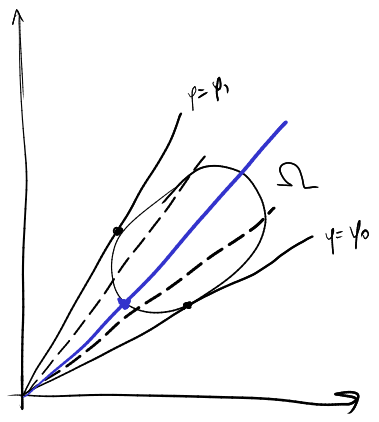
\includegraphics[scale=0.4]{3_1.png}
\end{center}
\begin{task}
\-
\begin{center}
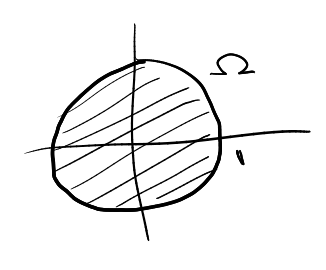
\includegraphics[scale=0.2]{3_2.png}
\end{center}
\[ \iint_\Omega f dx dy = \int^{2\pi}_0 d\varphi\int^1_0 f\cdot J\ dr \]
\end{task}
\begin{task}
\-
\begin{center}
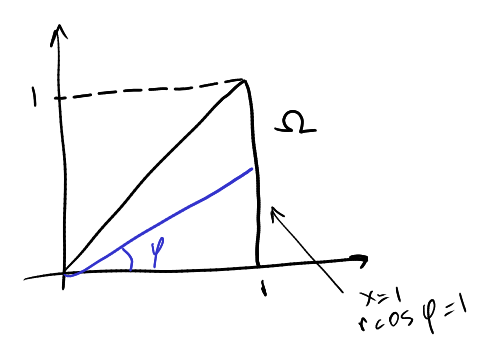
\includegraphics[scale=0.3]{3_3.png}
\end{center}
\[ \iint_\Omega f dx dy = \int^{\frac{\pi}{4}}_0 d\varphi \int_0^{\frac{1}{\cos\varphi}} dr\ f\cdot J = \int dr \int d\varphi\ f\cdot J \]
\end{task}
\begin{task}
\-
\begin{center}
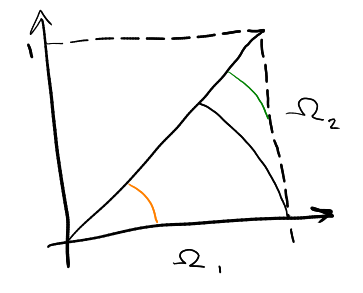
\includegraphics[scale=0.3]{3_4.png}
\end{center}
\[ \iint_\Omega f dx dy = \int^1_0 dr \int^{\frac{\pi}{4}}_0 d\varphi\ f\cdot J + \int_1^{\sqrt{2}}dr\int^{\frac{\pi}{4}}_{\arccos \frac{1}{2}}\]
\end{task}
\begin{task}
\-
\begin{center}
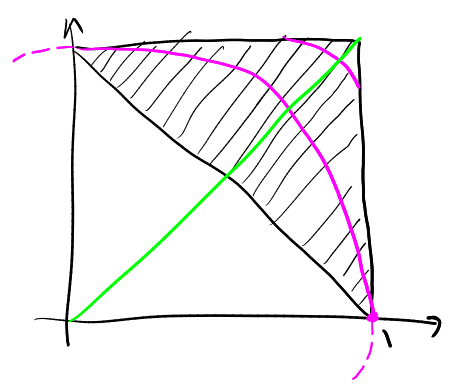
\includegraphics[scale=0.3]{3_5.png}
\end{center}
\[ \iint_\Omega = \int^{\frac{\pi}{4}}_0 d\varphi \int^{\frac{1}{\cos\varphi}}_{\frac{1}{\cos\varphi + \sin\varphi}} dr \dots + \int^{\frac{pi}{2}}_{\frac{\pi}{4}} d\varphi \int_{\frac{1}{\cos\varphi + \sin\varphi}}^{\frac{1}{\sin\varphi}} dr \dots = \]
\[ = \int_{\frac{\sqrt{2}}{2}}^1 dr \int \]
\end{task}
\begin{task}
\[ x^2 + y^2 \le \alpha x \]
\[ r = \alpha \cos\varphi \]
\[ \iint_\Omega = \int^{\frac{\pi}{4}}_{\frac{\pi}{4}}d\varphi\int^{\alpha\cos\varphi}_0 f\cdot J\ dr = \int^\alpha_0 dr \int^{\arccos \frac{\alpha}{2}}_{-\arccos \frac{\alpha}{2}} f\cdot J d\varphi \]
\end{task}
\section{Замена переменных}
\label{sec:org54d1cb7}
\begin{itemize}
\item \(x = x(u, v)\)
\item \(y = y(u, v)\)
\end{itemize}
\begin{center}
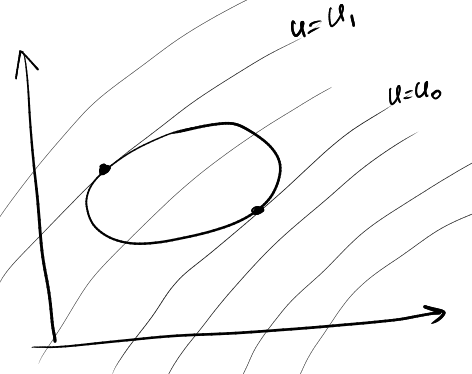
\includegraphics[scale=0.4]{3_6.png}
\end{center}
Фиксируем \(u = u_0\):
\[ \begin{cases}x = x(u_0, v) \\ y = y(u_0, v) \end{cases}\]
\[ \iint_\Omega f dx dy = \int_{u_0}^{u_1} du \int^{v_1(u)}_{v_0(u)} f(x(u, v), y(u, v)) \left(\det\begin{pmatrix}x'_u & x'_v \\ y'_u & y'_v \end{pmatrix}\right) dv \]
\[ \color{blue} \int f(x) dx = \int f(x(t)) x' dt \]
\end{document}
